\subsection{État du jeu}
Nous essaierons de simplifier au plus le jeu ``Candy Crush'' par l'utilisation de structures.\smallskip

Ce jeu comme beaucoup d'autres est jouable en niveaux qui sont caractérisés par certaines variables que nous présenterons ici :


\begin{typeag}[Niveau]
 -       \variable{numeroNiveau}{entier}{Les niveaux sont représentés par leur numéro (présent au départ)}\\
 -       \variable{deplacementMax}{entier}{Le nombre de déplacements maximum possibles selon le niveau}\\
 -       \variable{deplacementsUtilises}{entier}{Le nombre de déplacements effectués par l'utilisateur pendant la partie}\\
 -       \variable{grille}{[tailleX][tailleY]}{représente la grille d'entiers avec une taille en X et Y \\0 = case non jouable \\ 1,2,3,4,5 = couleur de bonbons }\\
 -       \variable{grilleDeDestruction}{booleen [tailleX][tailleY]}{est une seconde grille de booleens qui stocke les cases à détruire }
  \end{typeag}
  
  On crée un type agrégé représentant la position en x et y afin de cibler les cases plus tard :
  
  \begin{typeag}[Position]
 -       \variable{x}{entier}{position en x}\\
 -       \variable{y}{entier}{position en y}
  \end{typeag}
  
  La récompense du jeu se traduit par un score à obtenir afin de passer un niveau par exemple.
  Il nous faut donc une structure qui stocke le score que l'on doit obtenir pour gagner et aussi qui stocke le score actuel du joueur :
  
  \begin{typeag}[Score]
 -       \variable{cible}{entier}{score à atteindre (présent au début du niveau)}\\
 -       \variable{actuel}{entier}{stockage du score après chaque coup du joueur}
  \end{typeag}
  
  Quelques autres variables qui vont nous permettre de gérer le déplacement des cases et de vérifier la validité d'une combinaison :
  
\begin{typeag}[Case]
 -       \variable{caseTemporaire}{entier}{variable qui va stocker une case temporaire pour pouvoir inverser deux cases}\\
 -       \variable{nbCasesAlignes}{entier}{variable qui va compter le nombre de cases alignées}\\
 -		 \variable{caseADeplacer}{Position}{représente la position en x et y de la case que l'on souhaite déplacer}\\
 -       \variable{caseCible}{Position}{représente la position en x et y de la case que l'on cible}
 \end{typeag}

\subsection{Configuration initiale du jeu}
Nous allons maintenant analyser la situation de départ du jeu. Dès le départ, le joueur dispose d'un certain nombre d'éléments :

\begin{itemize}

\item
	Tout d'abord, le décor est constitué d'une grille modulable selon le niveau, c'est à dire avec une surface différente.
	Par exemple, on peut avoir une niveau assez simple (souvent au début) qui a une seule grille rectangulaire ou dans des niveaux plus complexes, plusieurs grilles avec des formes différentes.
\item
	Les bonbons qui constituent le jeu ont des couleurs qui vont permettre de faire des combinaisons.
	Couleurs : jaune, rouge, vert, bleu et orange.
\item
	À l'écran sera affiché le nombre de coups limite afin de réussir le niveau % On a enlevé le temps, je crois
\item
	Le joueur dispose aussi d'une jauge de points qui augmente au fur et à mesure des combinaisons.
	Évidemment, le score est 0 au départ.
\item
	Le joueur a aussi directement accès à son objectif à réaliser pour passer le niveau et son avancement dans celui-ci.
\item 
 	Pour que le jeu soit viable, il ne doit pas y avoir de combinaisons directes au départ (\emph{ex.: 3 bonbons alignés dès le début}).
	
\end{itemize}

\subsection{Évolution de l'état du jeu}

Le jeu consiste à déplacer deux éléments pour créer des alignements d'au moins 3 cases identiques. Pour ce faire, on va procéder en plusieurs étapes :

\subsubsection{Vérification du déplacement}
Avant de pouvoir échanger deux cases, il faut vérifier plusieurs choses :
\begin{itemize}
	\item
		Le déplacement ne sort pas de la grille
\begin{lstlisting}
caseDestination.x >= 0 && caseDestination.x < tailleX && caseDestination.y >= 0 && caseDestination.y < tailleY
\end{lstlisting}
	\item
		Le déplacement ne va pas sur une case non-jouable
\begin{lstlisting}
grille[caseDestination.x][caseDestination.y] != 0 && grille[caseADeplacer.x][caseADeplacer.y] != 0
\end{lstlisting}
	\item
		Les cases sont côtes à côtes (si on clique autre part, ça change la position de la caseADeplacer) :
\begin{lstlisting}
caseADeplacer.x - caseDestination.x == 1 || caseADeplacer.x - caseDestination.x == -1 || ( caseADeplacer.x - caseDestination.x != 1 && caseADeplacer.x - caseDestination.x != -1 && (caseADeplacer.y - caseDestination.y == 1 || caseADeplacer.y - caseDestination.y == -1) )
\end{lstlisting}
	\item
		Le déplacement va créer un alignement de au moins 3 cases identiques : pour cela, on va tout d'abord échanger les deux cases sélectionnées grace à la case temporaire :
\begin{lstlisting}
caseTemporaire = grille[caseDestination.x][caseDestination.y];
grille[caseDestination.x][caseDestination.y] = grille[caseADeplacer.x][caseADeplacer.y];
grille[caseADeplacer.x][caseADeplacer.y] = caseTemporaire;
\end{lstlisting}
		On peut alors commencer la détection des cases à détruire. Si il n'y a aucune case à détruire (lors de la première fois qu'on cherche), il n'y a donc pas de combinaison, on peut alors rééchanger les cases.
\end{itemize}

\begin{figure}[ht]
	\center
	\caption{\label{verifDepl} Déplacements}
	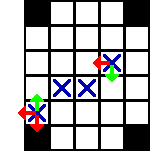
\includegraphics{imgs/verifDepl}
\end{figure}
		
\subsubsection{Détection}	
	
Pour pouvoir détecter toutes les cases à détruire, nous utilisons une autre grille de la même taille que celle contenant les éléments, mais cette nouvelle grille contient des booléens. Chaque case est ainsi associée à un booléen. Si la case doit être détruite, le booléens vaudra vrai.

On va ensuite parcourir la première grille ligne par ligne pour marquer tous les alignements horizontaux puis colonne par colonne pour les combinaisons verticales.

\begin{figure}[ht]
	\center
	\caption{\label{Detection} Détection}
	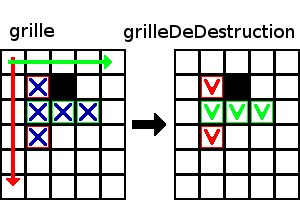
\includegraphics{imgs/Detection}
\end{figure}

Nous avons besoin de quelques nouvelles variables :

\begin{itemize}
\item
	couleurTemp, qui contient le numéro de couleur temporaire qui va servir pour verifier que plusieurs cases sont identiques;
\item
	nbCasesAlignees, qui sert a compter le nombre de cases alignees.
\end{itemize}

Après avoir initialisé les variables (à faire au début de chaque ligne, quand on parcours ligne par ligne, et au début de chaque colonne lorsqu'on parcoure colonne par colonne)
en mettant couleurTemp à la couleur de la première case de la ligne (respectivement de la colonne) et nbCasesAlignees à 1,
on va tester plusieurs choses :
\begin{itemize}
\item
	Si la couleur de la case visitée actuellement est la même que notre variable couleurTemp, on augmente nbCasesAlignees pour pouvoir compter le nombre de cases identiques à la suite.
\item
	Si la couleur est différente mais la variable nbCasesAlignées est supérieure ou égale à trois, ça signifie qu'il y a un alignement de au moins trois cases juste avant la case actuelle (non incluse).
	Dans ce cas, on va noter ces cases dans la seconde grille (avec i le numéro de colonne et j le numéro de ligne de la case en cours) :
\begin{lstlisting}
for(int k = i - nbCasesAlignees; k < i; k++)
{
	grilleDeDestruction[k][j] = true;
}
\end{lstlisting}
Il faudra également réinitialiser la couleur temporaire à la case actuelle et le compte des cases alignées à 1.
\item
	Si la couleur est différente, mais que nbCasesAlignees est inférieure à trois, c'est qu'aucun alignement n'était présent, on se contente donc de réinitialiser les variables (comme ci-dessus).
\item
	Enfin, il faut tester les alignements quand on est en fin de ligne (respectivement de colonne) : en effet, étant donné que les tests s'effectuent à la case suivant la fin de l'alignement, il faut en rajouter si
	l'on ne veut pas que les alignements au bord de grille soient oubliés.
	La condition ressemblera à ceci :
\begin{lstlisting}
if(i == tailleX - 1 && nbCasesAlignees >= 3)
\end{lstlisting}
	Afin d'utiliser la même fonction que celle qu'on utilisera pour noter les cases dans la seconde grille, on incrémentera i.
\end{itemize}

\subsubsection{Destruction}

Pour détruire les cases, nous remplaçons les cases à détruire par -1 dans la grille.

\begin{figure}[ht]
	\center
	\caption{\label{Destruction} Destruction}
	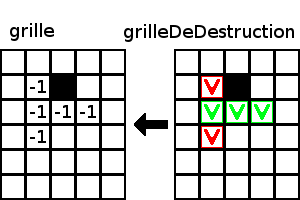
\includegraphics{imgs/Destruction}
\end{figure}

Cela se traduit comme suit :

\begin{lstlisting}
for(int j = 0; j < tailleY; j++)
{
	for(int i = 0; i < tailleX; i++)
	{
		if(grilleDeDestruction[i][j] == true)
		{
			grille[i][j] = -1;
			grilleDeDestruction[i][j] = false;
		}
	}
}
\end{lstlisting}

Après ça, la seconde grille aura retrouvé son état d'origine, c'est-à-dire avec des 'false' à chaque case.

\subsubsection{Remplacement}

	Afin de remplacer les cases détruites (donc -1 dans la grille), il faut trier la grille de manière à avoir tout les -1 au dessus.
	Il faut tout de même penser aux cases inutilisables (0 dans la grille) qui ne doivent pas être bougées.
	
	Nous allons donc parcourir chaque colonne en partant du bas, et lorsqu'on trouve un -1, nous allons le remplacer par la prochaine case valide (qu'on mettra à -1).
	
\begin{figure}[]
	\center
	\caption{\label{Remplacement} Remplacement}
	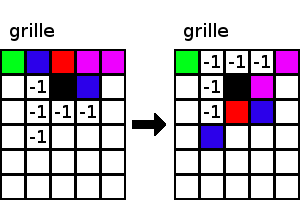
\includegraphics{imgs/Remplacement1}
	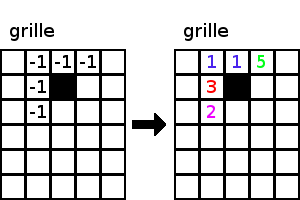
\includegraphics{imgs/Remplacement2}
\end{figure}
	
	Nous ajoutons deux variables : j qui servira à parcourir les cases à partir de celle où le programme se situe, et continuer qui est un boolen pour quitter la boucle en temps voulu.
	Pour une colonne k et une ligne i, nous aurons :
\begin{lstlisting}
if(grille[k][j] == -1) {
	j = i;
	continuer = true;
	while(j >= 0 && continuer == true)
	{
		j--;
		if(grille[k][j] != 0 && grille[k][j] != -1)
		{
			grille[k][i] = grille[k][j];
			grille[k][j] = -1;
			continuer = false;
		}
	}
}
\end{lstlisting}

	Ce comportement devra être effectué dans chaque case du tableau. Notons qu'on pourrais ajouter une condition qui arrêterais la boucle la première fois que le while ne trouve pas de case valide.
	
	Désormais, il ne reste plus qu'à remplacer toutes les cases -1 par un numéro aléatoire 1, 2, 3, 4 ou 5 représentant les différents types de cases, ce qui n'est pas compliqué car 
il suffit de parcourir chaque case de la grille et d'y insérer un entier aléatoire compris entre 1 et 5.

\begin{lstlisting}
for(int j = 0; j < tailleY; j++)
{
	for(int i = 0; i < tailleX; i++)
	{
		if(grille[i][j] == -1;
			grille[i][j] = (int)(Math.random() * 5) + 1;
	}
}
\end{lstlisting}

\subsubsection{Finalement}

Ce processus Détection-Destruction-Remplacement devra être répété jusqu'à ce qu'il n'y ait plus aucune case à détruire.

De plus, un score à atteindre pourra être fixé. Pour cela, chaque destruction de case (quand on les mets à -1) incrémentera d'un certain nombre de points la variable score.actuel. Le jeu pourra s'arrêter lorsque le score ciblé est atteint.
\begin{lstlisting}
score.actuel >= score.cible
\end{lstlisting}

Il est également possible de compter le nombre de coups que le joueur a utilisé. En effet, il suffit de le faire lors de l'échangement des cases. Si cet échange est par la suite annulé, le nombre de coups sera remis à son état d'avant l'échange.
Avec ceci, on peut définir un certain nombre de vies que le joueur possède, et qu'il perd à la perte d'un niveau, quand il n'a plus de vie, il doit attendre pour pouvoir continuer à jouer.
Enfin, lors du premier remplissage de la grille (un nombre aléatoire dans chaque case), il faudra éliminer toutes le combinaisons, c'est à dire lancer le processus Détection-Destruction-Remplacement autant de fois qu'il le faudra.

\subsection{Annexe}
Dans cette partie, nous ajouterons les analyses que nous avons pu faire sur \emph{Candy Crush} mais qui sont difficilement réalisables.
On peut compter parmi celles-ci les bonus qui s'obtiennent par certaines combinaisons de bonbons.
\begin{itemize}

\item
	Combinaison de 4 bonbons = un bonbon spécial qui détruit une ligne ou une colonne entière (selon le sens de ses rayures)
\item
	Combinaison de 5 bonbons = bombe multicolore (l'associer avec un autre bonbon détruit tout les bonbons du type associé présents dans la grille)
\item
	Bonbons spéciaux qui détruisent tout les bonbons autour d'eux : quand on fait deux combinaisons de 3 (en L)
\item
	Bonbons à retardement : vont exploser et détruire les bonbons autour d'eux 
\item
	Association de deux bonbons spéciaux pour un plus gros (détruit 3 lignes et 3 colonnes)      
\item
	Combos : une combinaison en entraîne d'autres (ajout de points)
\item
	Une combinaison détruit les bonbons et d'autres les remplacent (en tombant du dessus) % Edit pour l'overfull \hbox
\item
	Destruction automatique des bonbons spéciaux à la fin du niveau
\item
	Une solution au moins si on déplace un bonbon d'une case.
\end{itemize}
